\documentclass[]{upb_cs_thesis} % include german inside brackets for a German thesis

% load your own packages and user-defined commands
\usepackage[utf8]{inputenc}
\usepackage{latexsym}
\usepackage{amssymb}
\usepackage{amsmath}
\usepackage{amsfonts}
\usepackage{natbib}
\usepackage{graphicx}
\usepackage{sectsty}
\iffalse
\sectionfont{\fontsize{12}{14}\selectfont}
\fi
\sectionfont{\large}
\subsectionfont{\medium}
\newcommand{\newpar}{\vspace{.2in}\noindent}
\newcommand{\txti}{\textit}
\newcommand{\txtb}{\textbf}

%%%%%%%%%%
% Some commands for setting up theorem environments as provided by package 
% amsthm --- language sensitive
%%%%%%%%%
\theoremstyle{plain}
\newtheorem{definition}{Definition}[chapter]
\newtheorem{lemma}[definition]{Lemma}
\ifgerman
	\newtheorem{theorem}[definition]{Satz}
	\newtheorem{corollary}[definition]{Korollar}
	\newtheorem{example}[definition]{Beispiel}
\else
	\newtheorem{theorem}[definition]{Theorem}
	\newtheorem{corollary}[definition]{Corollary}
	\newtheorem{example}[definition]{Example}
\fi



%%%%%%%%%
% Your commands should go here...
%%%%%%%%%
\newcommand*{\eg}{e.\,g.}
\newcommand*{\ie}{i.\,e.}
\newcommand*{\cf}{c.\,f.}
\newcommand*{\etal}{et~al.}

\newacro{template}[UPB-CS-TT]{Paderborn University Computer Science thesis template}

\DeclareMathOperator{\testop}{top}



% set up some resources (graphics and bibliography)
\graphicspath{{figures/}}


%%%%%%%%%
% your thesis title, name, advisor, etc. go here;
%%%%%%%%%
\title{A Hybrid Graph Model for Distant Supervision Relation Extraction : A Report}
\author{Varun Maitreya Eranki}
\thesistype{Seminar Report}
%\thesistype{Bachelor's Thesis}
%\thesistype{Masterarbeit}
%\thesistype{Bachelorarbeit}
\degree{Seminar on}
%\degree{Bachelor of Science}
\researchgroup{DICE}
\supervisor{Diego Moussalem}
\submissiondate{\today{}}


% here your thesis really starts
\begin{document}

% start with the titlepage, the formalities, and then the abstract
% This file defines the title page of your thesis. You typically do not need to
% edit it. It is language sensitive and prints arguments passed to commands
% \author, \title, \thesistype, \degree, \researchgroup, \supervisor and
% \submissiondate, where required.
\begin{titlepage}
	\begin{center}
		\begin{minipage}{135mm}
			\hbadness=10000
			
\includegraphics[height=30mm]{figures/uni-logo}\\
			\ifgerman
				\textsf{
					\hspace*{20mm} Fakultät für Elektrotechnik,
					Informatik und Mathematik \\
					\hspace*{20mm} Institut für Informatik \\
					\hspace*{20mm} Arbeitsgruppe \theresearchgroup{} \\
				}
			\else
				\textsf{
					\hspace*{20mm} Faculty for Computer Science, 
					Electrical Engineering and Mathematics \\
					\hspace*{20mm} Department of Computer Science \\
					\hspace*{20mm} Research Group \theresearchgroup{} \\
				}
			\fi 
		\end{minipage}\\[40pt]

		{\huge \thethesistype{}}\\[5pt]
		\ifgerman
			Gerichtet an die Arbeitsgruppe \theresearchgroup{}\\
			zur Erreichung des Grades\\[5pt]
		\else
			Submitted to the \theresearchgroup{} Research Group\\
			in Partial Fullfilment of the Completion of\\[5pt]
		\fi 
		{\huge \thedegree{}}\\[30pt]

		{\Huge\textbf{\thetitle{}}}\\[30pt]

		\ifgerman
			von\\
		\else
			by\\
		\fi 
		{\Large\textsc{\theauthor{}}}\\[30pt]

		\ifgerman
			Betreut durch:\\
		\else
			Thesis Supervisor:\\
		\fi 
		{\large \thesupervisor{}}\\[30pt]

		Paderborn, \thesubmissiondate{}
	\end{center}
\end{titlepage}
 % prints the title page
% This is the legal statement
%  - that your thesis is a work of your own,
%  - that you have not used any source other than the ones you mention, 
%  - that you genuinely created your theses to achieve the desired academic
%    degree, and have not presented it to another examination board; and
%  - that you have clearly marked all concepts and ideas that you have adopted
%    from other works.
\chapter*{Erklärung}
	\thispagestyle{empty}
	Ich versichere, dass ich die Arbeit ohne fremde Hilfe und ohne
	Benutzung anderer als der angegebenen Quellen angefertigt habe und dass
	die Arbeit in gleicher oder ähnlicher Form noch keiner anderen
	Prüfungsbehörde vorgelegen hat und von dieser als Teil einer
	Prüfungsleistung angenommen worden ist. Alle Ausführungen, die wörtlich
	oder sinngemäß übernommen worden sind, sind als solche
	gekennzeichnet.\\
	\vspace{27pt}

	\begin{center}
		\begin{tabular}{l p{0.1\textwidth} r}
			\cline{1-1} \cline{3-3}
			\begin{minipage}[t]{0.4\textwidth}
				\centering
				Ort, Datum
			\end{minipage}
			&&  
			\begin{minipage}[t]{0.4\textwidth}
				\centering
				Unterschrift
			\end{minipage}
	\end{tabular}
\end{center}

 % prints the statement that you worked on your own and did not commit plagiarism
\cleardoublepage
\vspace*{\fill}
\begin{abstract}
	\noindent

Distant Supervision Relation Extraction (DSRE), supports users by providing automatically annotated data by using supervised and semi-supervised learning methods. A novel Hybrid Graph Model aids DSRE, by providing a framework for unsupervised learning methods. Limitations of other DSRE approaches are taken into consideration, and thereby, extended for different domains by incorporating heterogeneous background information. Previously, semi-supervised approaches incorporated, a specific type of background information depending, on a specific domain which achieved average results. As a downside, they cannot be extended to other domains and need customization. This novel approach generalizes the relation extraction problem. This approach outperforms, all other commonly used DSRE baseline approaches. It can be used with all models as it is flexible in embedding different kinds of domain information for relation extraction. Noisy data is gracefully handled in most cases using the built-in attention mechanism, that other approaches lack of. In \txti{"A Hybrid Graph Model for Distant Supervision Relation Extraction"}, authors \txti{Duan} et al., explores the benefits of using an Graph Convolution Networks with attention mechanism. Noisy data problem still persists and further evaluation of this method will yield, much better results in the future.
\end{abstract}
\vspace*{\fill}
\emptypage

\tableofcontents % prints the table of contents


%%%%%%%%%
% the contents of your thesis go into file body.tex
%%%%%%%%%
\chapter{Introduction}
\label{ch:introduction}

\newpar
From plain text, the task of extracting semantic relations between two or more entities, is known as Relation Extraction (RE). These relations can exist in different types. For example, \txti{"Germany is in Europe"} states a \txti{"is in"} relationship between \txti{"Germany"} and \txti{"Europe"}. With this information, a triple can be formed, \txti{<Germany, is in, Europe>}. Efficient RE is useful for applications like Knowledge Graph (KG) completion and question answering, which are in turn responsible for dependent applications. 


%%%%%add references %%%%%%%%%%
\newpar
Traditionally, supervised RE techniques produce elevated performance for RE\cite{bibid}. They solely rely on labeled data that is manually annotated. Manual annotation is time consuming and need an army of annotators. It is generally annotated into entities and relationships(entities: \txti{"Germany", "Europe"} relationship: \txti{"is in"}). This limitations strongly suggest need for semi-supervised or unsupervised RE techniques that are reliable enough and can mimic manual annotation. 

\newpar
Distant Supervision (DS) aims at solving this limitation by automatic production of labeled data by aligning KGs and plain text. In this process, it makes an assumption that, if there exists a relationship between two entities (\txti{e1, e2}) in Knowledge Base (KB), then all the sentences that consist \txti{e1, e2} express that relationship in some way\cite{zeng2015distant}. 
%%%use the same example of steve jobs%%%%%%

This introduces noise problem. It can be countered using Deep Neural Network (DNN) models, which try to provide a significant improvement, but fail in making predictions due to lack of sufficient background information associated with entities and relationships. For example, %%%%%%use steve jobs example%%%%%%
%%%%%%%%%%find citations%%%%%%%%%%
DNNs create bias at each stage and especially with long-tail relations, background information tend to be unusable for making predictions. They are mostly constructed for customized models to join knowledge that is limited to incorporate heterogeneous background information in parallel. Some of the methods did not handle the side effect caused due to introduced noise. 

%%%%%%%%introduce the topic%%%%%%%%%%


%\chapter{The upb\_cs\_thesis Document Class}
\label{ch:class_file}

In this section we discuss what the \emph{upb\_cs\_thesis} class as used by the
\acs{template} template does, and what commands and environments it provides.
We go through the file in chunks of lines that belong together and provide
descriptions afterwards.



\begin{verbatim}
\NeedsTeXFormat{LaTeX2e}
\ProvidesClass{ubp_cs_thesis}[2017/12/18 initial version]
\end{verbatim}

\vspace*{-6pt} \noindent
The \acs{template} template is requires the \LaTeXe{} and provides the
\emph{upb\_cs\_thesis} documents class



\begin{verbatim}
\newif\ifgerman\germanfalse
\DeclareOption{german}{\germantrue}
\end{verbatim}

\vspace*{-6pt} \noindent
The class supports English and German language options.
While the German language option (lower case: \emph{german}!) must be
explicitly requested, the class defaults to English.



\begin{verbatim}
\ProcessOptions
\LoadClass[a4paper, 11pt, twoside, openright]{book}
\end{verbatim}

\vspace*{-6pt} \noindent
The class is based on the standard book class provided by \LaTeX{}.



\begin{verbatim}
\ifgerman
        \RequirePackage[ngerman]{babel}
\else
        \RequirePackage[english]{babel}
\fi
\end{verbatim}

\vspace*{-6pt} \noindent
The class loads language packs depending on the language options passed to the
class.


\begin{verbatim}
\RequirePackage[T1]{fontenc}
\RequirePackage[utf8]{inputenc}
\RequirePackage{lmodern}
\RequirePackage{geometry}
\RequirePackage{graphicx}
\RequirePackage{hyperref}
\RequirePackage{csquotes}
\RequirePackage{tikz}
\RequirePackage{calc}
\RequirePackage[explicit]{titlesec}
\end{verbatim}

\vspace*{-6pt} \noindent
A couple of standard packages are loaded, for details on the packages, see
Section~\ref{sec:packages:class_packages}.



\begin{verbatim}
\reversemarginpar
\geometry{a4paper, twoside, left=30mm, right=20mm, top=30mm, bottom=30mm}
\end{verbatim}

\vspace*{-6pt} \noindent
The general page layout has 3cm margins on the top and bottom of an A4 page.
The inner margin is 3cm wide, while the outer one is 2cm wide.
The first page is to be considered a right page, \ie{} inner margins on the
left hand side of the page.



\begin{verbatim}
\pagestyle{empty}
\pagenumbering{roman}
\end{verbatim}

\vspace*{-6pt} \noindent
The first few pages of a thesis are not to show any headers or page numbers.
This behavior is altered in the \verb+\tableofcontents+ command.
Until then, page numbers are counted in Roman numbers, although only displayed
on the table of contents page.



\begin{verbatim}
\newcommand{\@upbchaptername}{}
\newcommand{\@upbsectionname}{}
\newcommand{\ps@upb}{%
  \renewcommand{\@oddhead}{\leftmark\hfill}%
  \renewcommand{\@evenhead}{\hfill\rightmark}%
  \renewcommand{\@oddfoot}{\hfill\thepage\hfill}%
  \renewcommand{\@evenfoot}{\hfill\thepage\hfill}%
}
\end{verbatim}

\vspace*{-6pt} \noindent
This class provides the \emph{upb} page style that prints the page number
centered et the bottom of the page and chapter or section number and name on
odd and even pages, respectively.


\begin{verbatim}
\newcommand*{\emptypage}{\newpage\null\thispagestyle{empty}\newpage}
\end{verbatim}

\vspace*{-6pt} \noindent
The class provides the \verb+\emptypage+ command that takes no argument and
adds an empty page to the document.



\begin{verbatim}
\newcommand{\thetitle}{undefined}
\newcommand{\theauthor}{undefined}
\let\oldtitle=\title
\let\oldauthor=\author
\renewcommand{\title}[1]{\renewcommand{\thetitle}{#1}\oldtitle{#1}}
\renewcommand{\author}[1]{\renewcommand{\theauthor}{#1}\oldauthor{#1}}
\newcommand{\thethesistype}{undefined}
\newcommand{\thedegree}{undefined}
\newcommand{\theresearchgroup}{undefined}
\newcommand{\thesupervisor}{undefined}
\newcommand{\thesubmissiondate}{undefined}
\newcommand{\thesistype}[1]{\renewcommand{\thethesistype}{#1}}
\newcommand{\degree}[1]{\renewcommand{\thedegree}{#1}}
\newcommand{\researchgroup}[1]{\renewcommand{\theresearchgroup}{#1}}
\newcommand{\supervisor}[1]{\renewcommand{\thesupervisor}{#1}}
\newcommand{\submissiondate}[1]{\renewcommand{\thesubmissiondate}{#1}}
\end{verbatim}

\vspace*{-6pt} \noindent
The class provides seven commands for setting data for a thesis title page:
\begin{enumerate}
	\item author: \verb+\author+,
	\item title: \verb+\title+,
	\item thesis type: \verb+\thesistype+,
	\item academic degree: \verb+\degree+,
	\item supervisor's research group name: \verb+\researchgroup+,
	\item supervisor's name: \verb+\supervisor+, and
	\item thesis submission date: \verb+\submissiondate+.
\end{enumerate}
These values passed to these commands can be accessed via commands
\begin{enumerate}
	\item \verb+\theauthor+,
	\item \verb+\thetitle+,
	\item \verb+\thethesistype+,
	\item \verb+\thedegree+,
	\item \verb+\theresearchgroup+,
	\item \verb+\thesupervisor+, and
	\item \verb+\thesubmissiondate+, respectively.
\end{enumerate}
\noindent Since \verb+\author+ and \verb+\title+ commands are provided by
\LaTeX{} by default, we change their behavior slightly to make the values
passed to the commands available in a manner consistent with the other
commands, but we also preserve their original behavior.

These commands are used to typeset the title page as defined in
\mbox{pretext/titlepage.tex}



\begin{verbatim}
\newenvironment{abstract}{
    \begin{center}
        \begin{minipage}{.9\textwidth}
            \ifgerman
                \textbf{Zusammenfassung.} \hspace*{0.10pt}
            \else
                \textbf{Abstract.} \hspace*{0.10pt}
            \fi
}{
        \end{minipage}
    \end{center}
}
\end{verbatim}

\vspace*{-6pt} \noindent
The class provides the language sensitive \verb+abstract+ environment for
typesetting an abstract for your thesis.



\begin{verbatim}
\let\@upbtocold=\tableofcontents
\renewcommand{\tableofcontents}{
  \pagestyle{plain}	
  \@upbtocold
  \cleardoublepage
  \setcounter{page}{0}
  \pagestyle{upb}
  \pagenumbering{arabic}
  \renewcommand{\chaptermark}[1]{
    \markboth{\rm\chaptername\ \thechapter.\ #1}{}
  }
  \renewcommand{\sectionmark}[1]{
    \markright{\rm\thesection\ #1}{}
  }
}
\end{verbatim}

\vspace*{-6pt} \noindent
Starting with the table of contents, the thesis page numbers are displayed
(Roman numbers).
After the table of contents, page numbers are reset to 0, displayed in Arabic, 
and headers (lowercase upright chapter and section names) are shown. 
For this the behavior of \verb+\tableofcontents+ is altered, but its original
behavior is preserved.



\begin{verbatim}
\newlength{\@upbchapternumberwidth}
\newlength{\@upbtitlemaxwidth}
\newlength{\@upbtitletextwidth}
\end{verbatim}

\vspace*{-6pt} \noindent
These are some dimensions used by the upcoming commands to layout chapter
openings.



\begin{verbatim}
\titleformat{\chapter}{
  \normalfont\huge\bfseries
}{}{0em}{
  \newcommand*{\@upbprintscaledchapternumber}{
    \resizebox{!}{15mm}{\thechapter}
  }   
  \settowidth{\@upbchapternumberwidth}{
    \@upbprintscaledchapternumber
  }   
  \setlength{\@upbtitlemaxwidth}{
    .9\textwidth - \@upbchapternumberwidth 
  }   
  \settowidth{\@upbtitletextwidth}{#1}
  \flushright
  \rlap{
    \parbox[b]{\textwidth + 23mm}{
      \parbox[b]{\@upbtitlemaxwidth}{
        \ifdim\@upbtitletextwidth<\@upbtitlemaxwidth
          \hfill #1
	\else
          #1\hbadness=10000
        \fi 
      }   
      \hspace{12mm}
      \makebox[\@upbchapternumberwidth][b]{
        \raisebox{12mm}{\@upbprintscaledchapternumber}
      }   
      \hspace{-\@upbchapternumberwidth}
      \hspace{-12mm}
      \begin{tikzpicture}
        \fill[black] (0mm, 0mm) rectangle
           (\@upbchapternumberwidth +23mm, 10mm);
      \end{tikzpicture}
    }   
  }   
}
\end{verbatim}

\vspace*{-6pt} \noindent
These lines define the layout of a numbered chapter opening:
the chapter name to the left of a black box, the chapter number atop the bar.
The first few lines compute the width of the printed chapter number, and the
text available for the chapter name.
The width of the black box depend on the width of the chapter number, so we
account for arbitrary digit numbers.
If the chapter name is wide than the space available, line breaks are
automatically applied, the name becomes left aligned, and the base line of its
lowest line is the bottom line of the black box.
If there is sufficient space, the text is right aligned.



\begin{verbatim}
\titleformat{name=\chapter,numberless}{
  \normalfont\huge\bfseries
}{}{0em}{
  \settowidth{\@upbchapternumberwidth}{
    \resizebox{!}{15mm}{0}
  }   
  \setlength{\@upbtitlemaxwidth}{
    .9\textwidth - \@upbchapternumberwidth 
  }   
  \settowidth{\@upbtitletextwidth}{#1}
  \flushright
  \rlap{
    \parbox[b]{\textwidth + 23mm}{
      \parbox[b]{\@upbtitlemaxwidth}{
        \ifdim\@upbtitletextwidth<\@upbtitlemaxwidth
          \hfill
	\else
          #1  
        \fi 
      }   
      \hspace{8mm}
      \begin{tikzpicture}
        \fill[black] (0mm, 0mm) rectangle
            (\@upbchapternumberwidth +23mm, 10mm);
      \end{tikzpicture}
    }
  }
}
\end{verbatim}

\vspace*{-6pt} \noindent
This is a version of the chapter opening for unnumbered chapters.



\begin{verbatim}
\titlespacing*{\chapter}{0pt}{30pt}{25pt}
\end{verbatim}

\vspace*{-6pt} \noindent
This command sets the spacing around chapter openings; it is required by the
\emph{titlesec} package.

\chapter{Concepts}
\label{ch:concepts}

\chapter{Architecture}
\label{ch:architecture}

Architecture of Hybrid Graph Model is shown in Fig.\ref{fig:arch}. This can be broadly divided into three segments. First segment consists of information encoders with individual encoders for various levels of data. Second or Middle segment consists of hybrid KG. This graph is constructed, by utilizing vector representations generated by encoders in previous step, and embedding them as, individual piece of information in a node that is relevant. In the Final segment, this hybrid graph is utilized by GCN with attention to extract features of the hybrid KG and final output is a probability distribution of the relations. The author, S. Duan et al.\cite{duan2019hybrid}, proposes to predict the relation between any entity pair $S_{(x_i, y_i)}$ and learn the probability distribution $P(r_i|x_i,y_i;\theta)$ over all relations $r_i \in \mathbb{R}$, where $\theta$ denotes the parameters of the model.

\begin{figure}[h!]
	\centering
	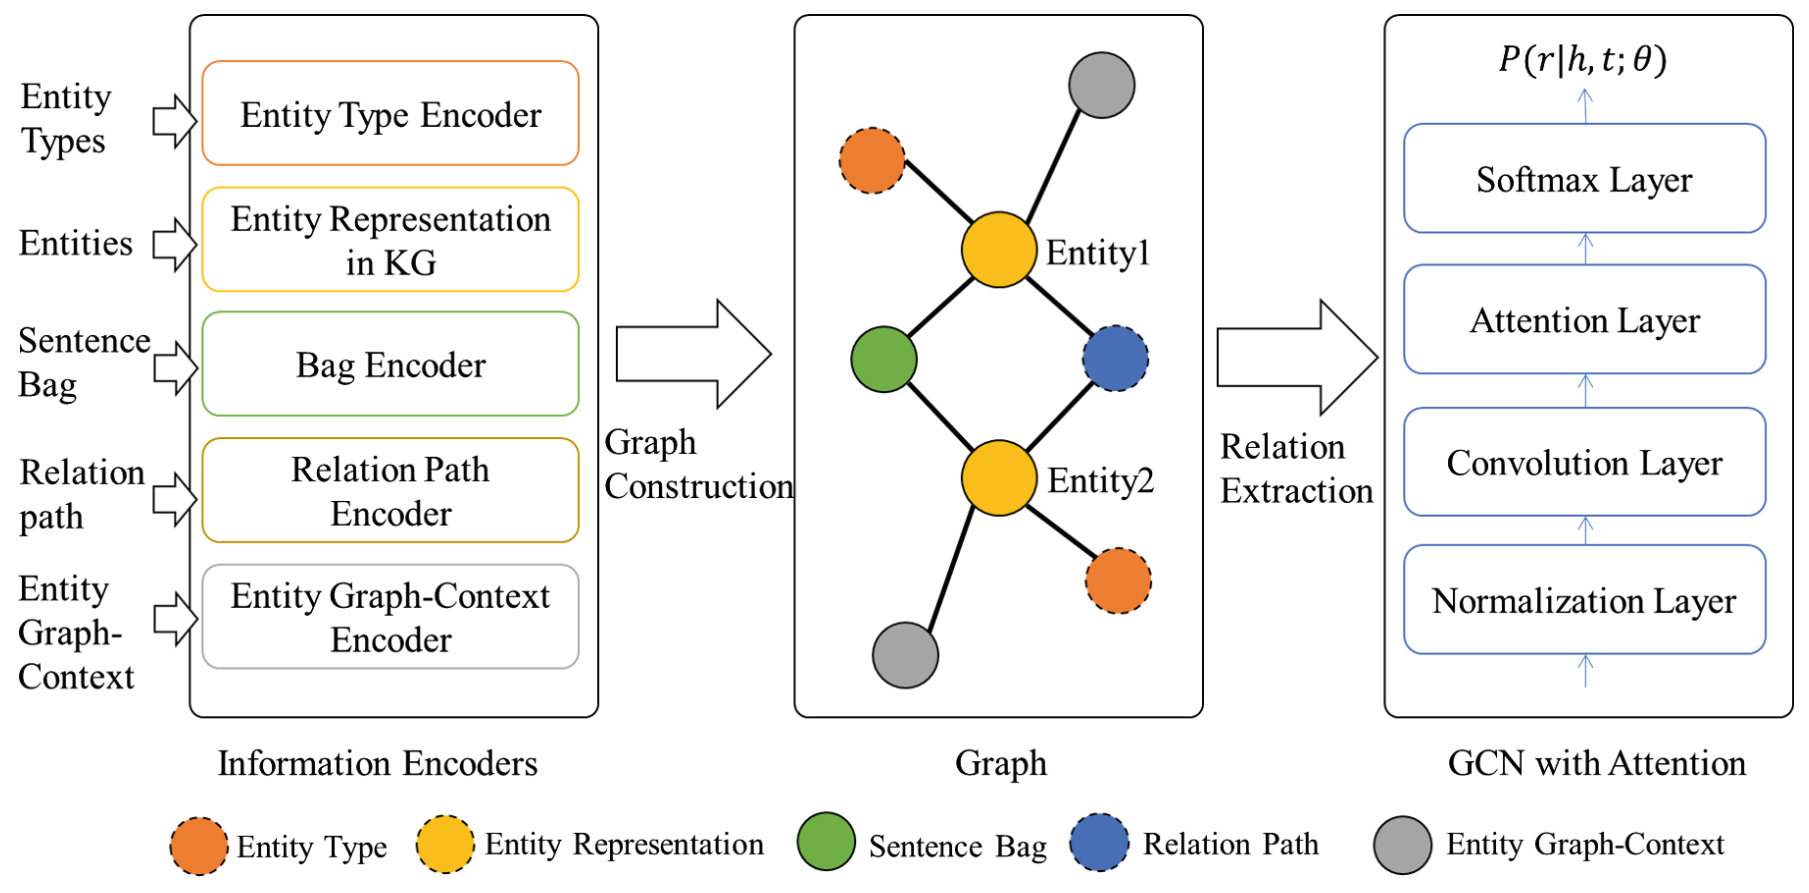
\includegraphics[scale=0.25]{figures/architecture.PNG}
	\caption{The Architecture}
	\label{fig:arch}
\end{figure}

\newpar
Before the process, from a given DS generated data set $D = \{S_{(x_i,y_i)}|,i = 1,2,...\}$, the background information from KG for every entity pair $(x_i, y_i)$ is extracted and stored in a different data set $\mathbb{I} = \{I_{(x_1,y_1)},I_{(x_2,y_2)},...\}$. Label of each instance corresponds to the label of $S_{(x_i, y_i)}$ during the extraction. 




\begin{figure}[h!]
	\centering
	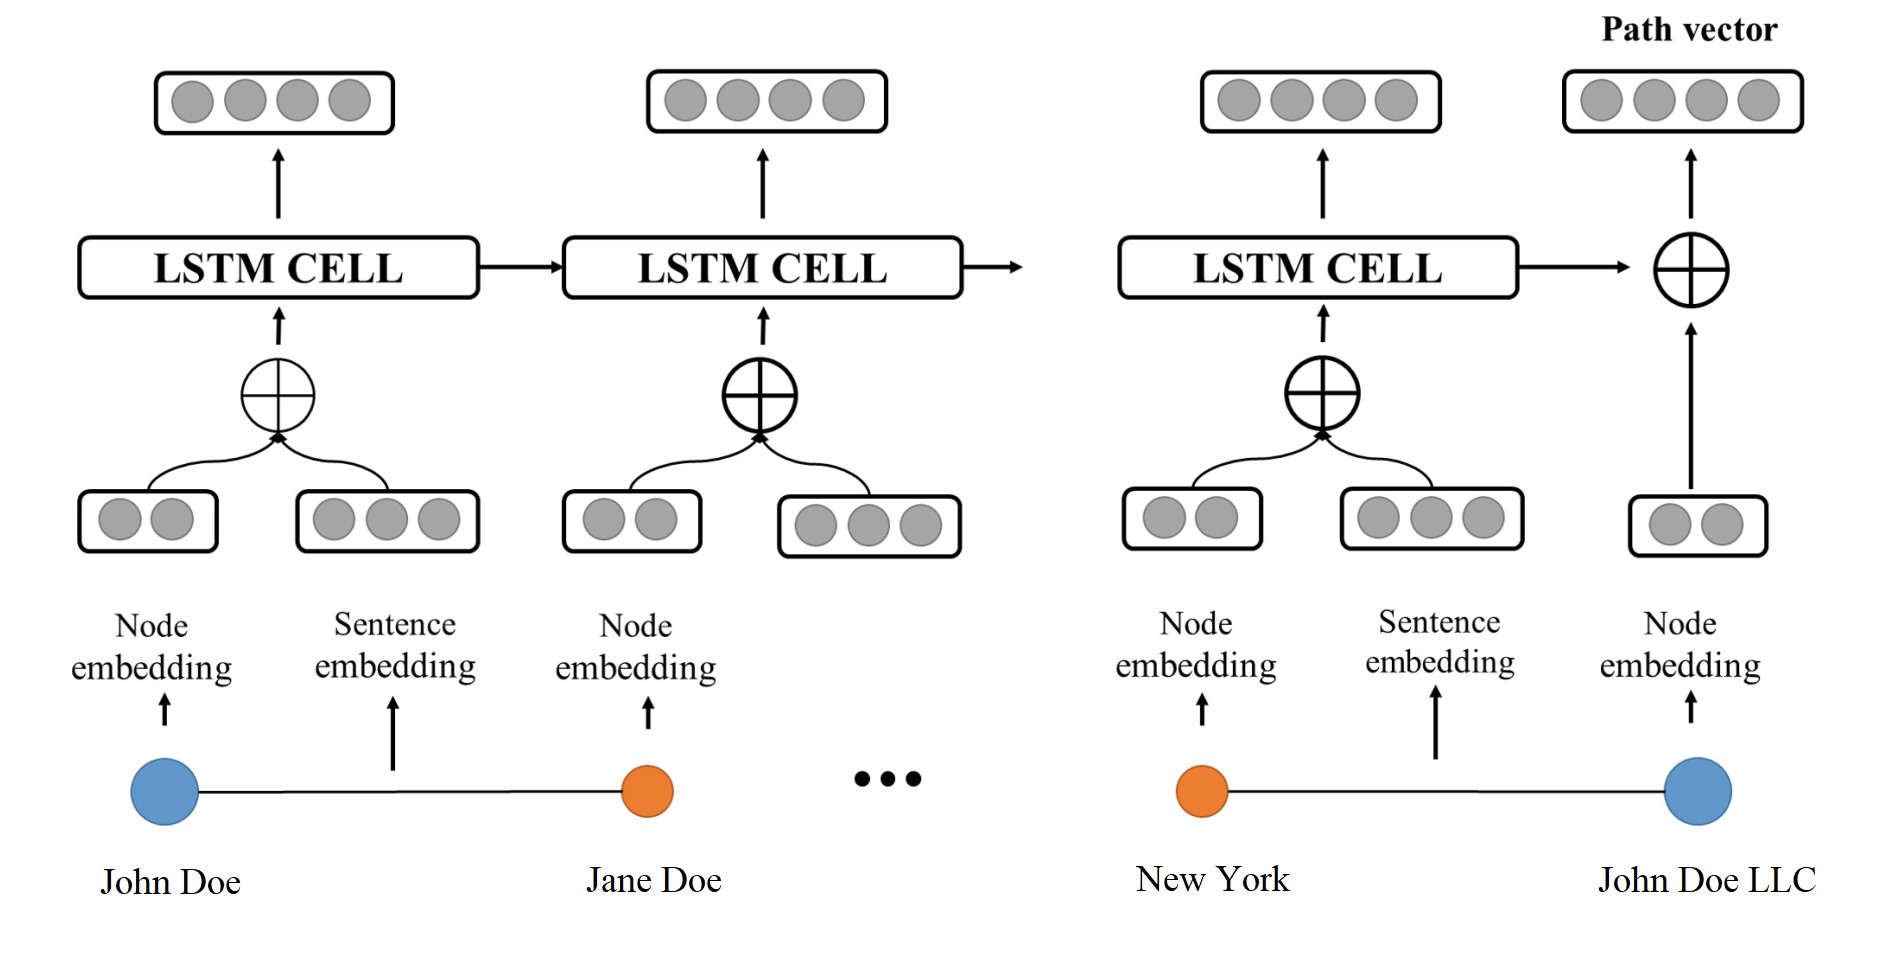
\includegraphics[scale=0.2]{figures/LSTM.PNG}
	\label{fig:lstm}
\end{figure}
\chapter{Discussion}
\label{ch:discussion}

Convolutional neural networks serve as a powerful tool to solve high dimensional problems. CNNs give good results when, used with euclidean data (images, videos, sounds) that are compositional. Compositional features can be extracted and fed to a classifier, etc. These can be represented using euclidean domain that are regular spatial structures (for Eg. distance of adjacent pixels in an image are the same). To learn from non-euclidean data (real world data) like social networks web, Knowledge Graphs, etc. which are in the form of graphs, CNNs are adapted into Graph Convolutional Neural Networks (GCNs). They are similar to CNNs, but, instead of aggregating individual weights (distance of a node to adjacent nodes), a single shared weight is used by approximation. This solves the limitations of CNNs when nodes have non uniform neighbors. Most DSRE approaches are aimed towards semi-supervised models\cite{smirnova2018relation}. The authors Duan et al.\cite{duan2019hybrid}, aims to show that GCNs are useful for unsupervised DSRE. Limitations of semi-supervised model proposed by Kipf et al.\cite{kipf2016semi}, have been overcome with this HG model.

\newpar
Proposed HG model is based on models proposed by Daojian Zeng et al.,\cite{zeng2014relation} and Wenyuan Zeng et al.,\cite{zeng2016incorporating}. In a novel way, incorporating relation path information in neural RE show a baseline results of efficient DSRE. Common limitation in dealing with non-euclidean data is noise problem. There are standard methods to solve noise problem for euclidean data\cite{zimek2012survey}, but not for the later case. Authors Duan et al.,\cite{duan2019hybrid} uses an attention mechanism by selecting more relevant features to reduce the affect of noise using weighted sum operation over all features. Higher weight is assigned to important features, and can be altered to select or deselect those features that have high noise. Noise is a vague concept. To understand noise, let us consider two features, entity types and relations. For a certain use-case, that has more information on relations, but not much information about entity types. Model is said to have more noise, if entity types feature is given more weight. Prediction based on such training data would be less efficient. This feature of GCNs is used in HG model, which yields higher precision compared previous approaches. Compared to previous approaches, feature information is encoded using various feature encoders and the resultant eigen vectors(simply vectors) are embedded into hybrid graph. This embedding also embeds noisy data during encoding phase, that gets carried on to next step. The only way of controlling the affects of noise is using weight mechanism in attention layer for a hidden layer of GCN. This improves the precision but does not completely eliminate the noise problem which is the suggested future work.

\newpar
One major achievement in HG model is, fusing heterogeneous information from the feature encoders, into a single hybrid graph, as they have different vector embedding. Where each vector represents a node in the graph. An adjacency matrix is used to explain the correlation between nodes. For each instance, and each vector embeddings, this varying structure is converted into a fixed structure using adjacent matrix. Then, high-level features are extracted by using GCN. The training phase for huge corpus takes a very large time. Decent sized dataset was used by aligning Wikidata relations with New York Times Corpus (NYT) for PCCNs\cite{zeng2016incorporating}. Wikidata has more than 80 million triple facts and 20 million entities which is a large sample size to do training. The experimental setup used for PCCNs is used as is, with small changes in parameters like learning rate for SGD, word embedding size, etc. This will not affect the overall results as main goal was comparison. Core advantage of deep learning techniques is, less time for testing phase. Other machine learning techniques which try to learn based on existing data take less training time and more testing time. Authors Duan et al.,\cite{duan2019hybrid} discusses about run-time in less detail as it is prevalent that run-time depends on configuration of machine used, so not applicable in this case. 

\newpar
Authors Duan et al.,\cite{duan2019hybrid} discusses about examples of testing dataset that do not occur. Using long-tail relations, HG model is able to out perform other models and find some score where other models fail. This proves authors' assumption that, embedding additional information apart from a specific feature will yield better results for unseen data. 
\chapter{Results and Comparisons}
\label{ch:resultscomparisons}

\newpar


%\input{chapters/evaluation}
\chapter{Conclusion and Future work}
\label{ch:conclusion}

To conclude, authors \txti{S. Duan} et al.\cite{duan2019hybrid}, in the work \txti{“A Hybrid Graph Model for Distant Supervision Relation Extraction”} propose a novel and different approach to incorporate heterogeneous information for DSRE. For this model, the core principles of semi-supervised learning models borrowed and their limitations we eliminated to a great extent. The vector representation of data enable to hand-pick specific features, by a simple aggregated weight mechanism at each level. Memory over-head to store large graphs is completely eliminated. A real-world data-set was chosen, and this approach achieves better results. Authors claim that the approach works best for known good data, and manages to find a long-tail relation for unseen data. Claims were also made that, this approach is applicable to any type of unstructured data in all application domains. The proposed technique should be explored further over other application domains to prove the claims. The future work comprises of reduction of noisy data. Data-sets with particularly sparse graphs should be chosen, to find a specific pattern, to alleviate the noisy data completely. The authors intend to solve this problem by devising an efficient method, along with generalizing this approach to large unlabeled text for learning more confident information. 



% include the bibliography, and add it as a chapter the table of contents
\newpage
\addcontentsline{toc}{chapter}{Bibliography}
\bibliographystyle{alpha}
\bibliography{literature.bib}


%%%%%%%%%
% the appendices of your thesis go into file appendix.tex
%%%%%%%%%
\appendix



\end{document}
